\documentclass{standalone}
\usepackage{pgfplots}


\xdefinecolor{redx}{rgb}{1,0,0}
\xdefinecolor{greenx}{rgb}{0,.7,0}
\xdefinecolor{bluex}{rgb}{0,0,.8}
\xdefinecolor{purplex}{rgb}{.7,0,.7}
\xdefinecolor{orangex}{rgb}{.9,.5,0}

\newcommand{\rgrey}[1]{{\color{greyx!40}#1}}
\xdefinecolor{greyx}{rgb}{0,0,0}

\newcommand{\rred}[1]{{\color{redx!100}#1}}
\newcommand{\ggreen}[1]{{\color{greenx!100}#1}}
\newcommand{\bblue}[1]{{\color{bluex!100}#1}}
\newcommand{\ppurple}[1]{{\color{purplex!100}#1}}
\newcommand{\oorange}[1]{{\color{orangex!100}#1}}
\renewcommand{\vec}{\mathbf}

\begin{document}

\begin{tabular}{cc}

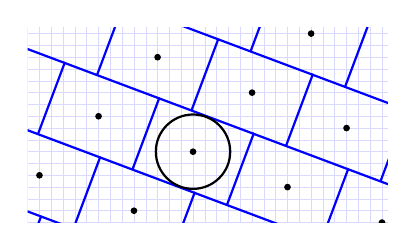
\begin{tikzpicture}[scale=.15]
  \clip(-4,4)  rectangle (26.5,20.5);
   \coordinate (Origin) at (0,0); 
   \coordinate (Bone) at (8,-3);
   \coordinate (Btwo) at (5,5);
   \coordinate (p) at (12,12);
   \coordinate (v) at (10,10);
     \draw[style=help lines,color=blue!15] (-6,4) grid[step=1cm] (27,21);
%     \draw[style=help lines,thin,dotted] (-9,-9) grid[step=1cm] (23,23);
  \node[draw,circle,inner sep=2pt] at (0,0) {};     
% \draw [very thick,-latex,blue] (Origin)    -- (Bone) node [left] {$\vec b_1$};
%     \draw [very thick,-latex,blue] (Origin)   -- (Btwo) node [left] {$\vec b_2$};
  \foreach \y in {-3,-2,...,5}{%Two indices running over each 
      \foreach \x in {-3,-2,...,5}{% node on the grid we have drawn
    \node[draw,circle,inner sep=.7pt,fill] at (8*\x-3*\y,-3*\x+8*\y) {};
    \draw[blue,thick] 
          (8*\x-3*\y - 165/146 - 8/2,-3*\x+8*\y - 440/146 + 3/2)  --
          (8*\x-3*\y + 165/146 - 8/2,-3*\x+8*\y + 440/146 + 3/2)  --
          (8*\x-3*\y + 165/146 + 8/2,-3*\x+8*\y + 440/146 - 3/2);

    
    }
}
\node[draw, thick, circle,inner sep=9.5] at (10,10) {};
 \end{tikzpicture}
&
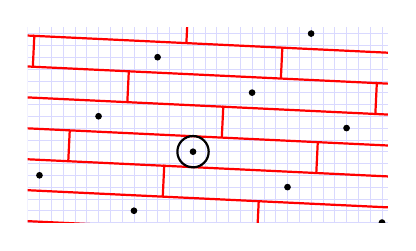
\begin{tikzpicture}[scale=.15]
  \clip(-4,4)  rectangle (26.5,20.5);
   \coordinate (Origin) at (0,0); 
   \coordinate (Bone) at (21,-1);
   \coordinate (Btwo) at (13,2);
   \coordinate (Btwos) at (55/442,1155/442);
   \coordinate (p) at (12,12);
   \coordinate (v) at (23,12);
     \draw[style=help lines,color=blue!15] (-6,4) grid[step=1cm] (27,21);
 %    \draw[style=help lines,thin,dotted] (-9,-9) grid[step=1cm] (23,23);
  \node[draw,circle,inner sep=2pt] at (0,0) {};     
% \draw [very thick,-latex,red] (Origin)    -- (Bone) node [below] {$\vec b_1$};
%     \draw [very thick,-latex,red] (Origin)   -- (Btwo) node [above] {$\vec b_2$};
  \foreach \y in {-3,-2,...,5}{%Two indices running over each 
      \foreach \x in {-3,-2,...,6}{% node on the grid we have drawn
    \node[draw,circle,inner sep=.7pt,fill] at (8*\x-3*\y,-3*\x+8*\y) {};
    \draw[red,thick]  
          (8*\x-3*\y - 55/884 - 21/2,-3*\x+8*\y - 1155/884 + 1/2)  --
          (8*\x-3*\y + 55/884 - 21/2,-3*\x+8*\y + 1155/884 + 1/2)  --
          (8*\x-3*\y + 55/884 + 21/2,-3*\x+8*\y + 1155/884 - 1/2);
    }
    }
    \node[draw, thick, circle,inner sep=4] at (10,10) {};
 \end{tikzpicture} \\
  Decoding radius with $\vec G^\star$ & Decoding radius with $\vec B^\star$
\end{tabular}



\end{document}
